\documentclass[a4paper,12pt]{article}
%%%%%%%%%%%%%%%%%%%%%%%%%%%%%%%%%%%%%%%%%%%%%%%%%%%%%%%%%%%%%%%%%%%%%%%%%%%%%%%%%%%%%%%%%%%%%%%%%%%%%%%%%%%%%%%%%%%%%%%%%%%%%%%%%%%%%%%%%%%%%%%%%%%%%%%%%%%%%%%%%%%%%%%%%%%%%%%%%%%%%%%%%%%%%%%%%%%%%%%%%%%%%%%%%%%%%%%%%%%%%%%%%%%%%%%%%%%%%%%%%%%%%%%%%%%%
\usepackage{eurosym}
\usepackage{vmargin}
\usepackage{amsmath}
\usepackage{graphics}
\usepackage{framed}
\usepackage{epsfig}
\usepackage{subfigure}
\usepackage{fancyhdr}

\setcounter{MaxMatrixCols}{10}
%TCIDATA{OutputFilter=LATEX.DLL}
%TCIDATA{Version=5.00.0.2570}
%TCIDATA{<META NAME="SaveForMode"CONTENT="1">}
%TCIDATA{LastRevised=Wednesday, February 23, 201113:24:34}
%TCIDATA{<META NAME="GraphicsSave" CONTENT="32">}
%TCIDATA{Language=American English}

\pagestyle{fancy}
\setmarginsrb{20mm}{0mm}{20mm}{25mm}{12mm}{11mm}{0mm}{11mm}
\lhead{MA44128} \rhead{Data Modelling} \chead{Midterm
	Part A Review Questions } %\input{tcilatex}
\begin{document}
\section*{Part A Revision Questions}
\subsection*{Q1. Theory for Inference Procedures (3 Marks)}
Answer the three short questions. Each correct answer will be awarded 1 mark.
\begin{itemize}
 \item[i.] What is a $p-$value?
\item[ii.] Briefly describe how $p-$value is used in hypothesis testing
\item[iii.] What is meant by a Type I error?
\item[iv.] What is meant by a Type II error?
\end{itemize}
% -- Part 1 - Theory
%
% 1 Mark What is a $p-$value
% 1 Mark Briefly describe how $p-$value is used in hypothesis testing
% 1 Mark Type I error
% 1 Mark Type II error
% 2 Marks A data set is determined to be not normally distributed. Briefly describe two operations that can typically be performed in this instance.
% -- Log Transformation
% -- Test for Outliers
% 1 Mark Non Parametric Inference
% -- Marks Tally so far 7 Marks

%\newpage
\subsection*{Q2. Normal Distribution (6 Marks)} % Normal %6 MARKS
Assume that the diameter of a critical component is normally distributed with a Mean of 50mm and a Standard Deviation of 2mm. You are required  to estimate the approximate probability of the following measurements occurring on an individual component.
\begin{itemize}
	\item [i.](2 Marks)	Between 50 and 51.2mm
	\item [ii.](2 Marks) Less than 48.5 mm
	\item [iii.](2 Marks) Between 48.2 and 51.6 mm
\end{itemize}

\noindent Use the normal tables to determine the probabilities for the above exercises. You are required to show all of your workings.

\subsection*{Q3. Dixon Q Test For Outliers (4 Marks)}

The typing speeds for one group of 12 Engineering students were recorded both at the beginning of year 1 of their studies. The results (in words per minute) are given below:

\begin{center}
\begin{tabular}{|c|c|c|c|c|c|c|}
\hline
% Subject& A& B& C& D& E &F &G &H \\ \hline
121 & 146 & 150 &149 &142 &170& 153\\ \hline
 137 & 161 & 156& 165& 137& 178& 159
\\ \hline
\end{tabular}
\end{center}
Use the Dixon Q-test to determine if the lowest value (121) is an outlier. You may assume a significance level of 5\%.
%Calculate a 95\% confidence interval for the difference between the mean number of marks obtained by males and females in the population of school leavers as a whole.
%(7 marks)

\begin{itemize}
\item[i.] (1 Mark) Formally state the null hypothesis and the alternative hypothesis.
\item[ii.] (1 Mark) Compute the Test Statistic.
\item[iii.] (2 Mark) By comparing the Test Statistic to the appropriate Critical Value, state your conclusion for this test.
\end{itemize}

\subsection*{Q4. Testing Normality (2 Marks)} %4 Marks
A graphical procedure was carried out to assess whether or not this assumption of normality is valid for data set \texttt{Y}. Consider the Q-Q plot in the figure below.

\begin{center}
	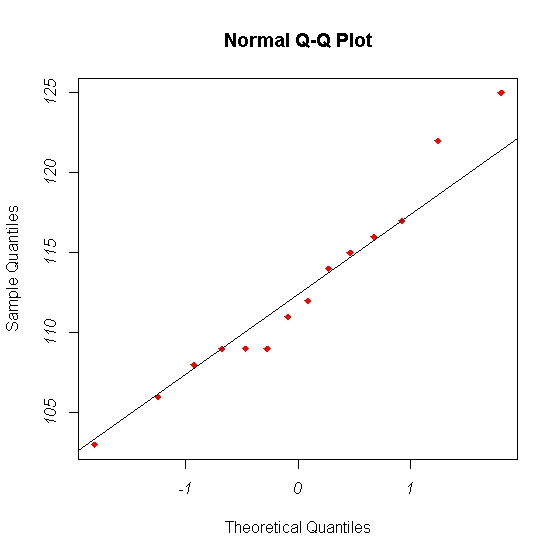
\includegraphics[scale=0.45]{images/Q5examQQplot}
\end{center}

\begin{itemize}
	\item[i.] (1 Mark) Provide a brief description on how to interpret this plot.
	\item[ii.] (1 Mark) What is your conclusion for this procedure? Justify your answer.
\end{itemize}
\newpage
\subsection*{Q5. Testing Normality (3 Marks)} %4 Marks
Consider the following inference procedure performed on data set $X$.
\begin{center}
	\begin{verbatim}
	> shapiro.test(X)
	
	Shapiro-Wilk normality test
	
	data:  X
	W = 0.9619, p-value = 0.6671
	
	\end{verbatim}
\end{center}


\begin{itemize}
	\item[i.] (1 Mark) Describe what is the purpose of this procedure.
	\item[ii.] (1 Mark) What is the null and alternative hypothesis?
	\item[iii.] (1 Mark) Write the conclusion that follows from it.
\end{itemize}

\subsection*{Q6. Testing For Outliers (6 Marks)}
\begin{itemize}
	\item[(i)] (3 Marks) Provide a brief description for three tests from the family of Grubb's  Outliers Tests. Include in your description a statement of the null and alternative hypothesis for each test, any required assumptions and the limitations of these tests.
	\item[(ii)] (3 Marks) Showing your working, use the Dixon Q Test to test the hypothesis that the maximum value of the following data set is an outlier.
	\[ 19,22,23,24,25,26,29,38\]
\end{itemize}

\newpage
\subsection*{Q7. Testing for Outliers (3 Marks)} %4 Marks
The following statistical procedure is based on this dataset.
\begin{center}
\begin{tabular}{|cccc|}
	\hline
	% after \\: \hline or \cline{col1-col2} \cline{col3-col4} ...
	6.98 &8.49 &7.97& 6.64\\
	8.80 &8.48 &5.94& 6.94\\
	6.89 &7.47 &7.32& 4.01\\
	\hline
\end{tabular}
\end{center}

\begin{framed}

	\begin{verbatim}
	> grubbs.test(x, two.sided=T)
	
	Grubbs test for one outlier
	
	data:  x
	G = 2.4093, U = 0.4243, p-value = 0.05069
	alternative hypothesis: lowest value 4.01 is an outlier
	\end{verbatim}
\end{framed}

\begin{itemize}
	\item[i.] (1 Mark) Describe what is the purpose of this procedure. State the null and alternative hypothesis.
	\item[ii.] (1 Mark) Write the conclusion that follows from it.
	\item[iii.] (1 Mark) State any relevant assumptions for this procedure.
\end{itemize}
\subsection*{Q8. Numeric Transformation of Data} %4 Marks


\begin{itemize}
	\item[(i)] Describe the purpose of transformations
	\item[(ii)] Describe the process of transformations
	\item[(iii)] Describe the purpose of Tukey's Ladder (referencing direction and relative strength)
	\item[(iv)] Give an example of a transformation for various types of skewed data (use Tukey's Ladder, with an example for both directions)
	\item[(v)] Describe the limitations of transformations
\end{itemize}
\newpage
\subsection*{Q9. - Control Limits }

\begin{framed}
	Exam Paper Formulas for Control Limits
	\begin{itemize}
		\item Process Mean
		
		
		
		\[ \bar{\bar{x}} \pm 3\frac{\bar{s}}{c_4\sqrt{n}}\]
		\item Process Standard Deviation	
		\[ \bar{s} \pm 3\frac{c_5\bar{s}}{c_4}\]
		\item Process Range	
		\[\left[ \bar{R}D_3, \bar{R}D_4\right]\]
	\end{itemize}	
\end{framed}



A normally distributed quality characteristic is monitored through the use of control charts. These charts have the following parameters. All charts are in control.
\begin{center}
	\begin{tabular}{|c|c|c|c|}
		\hline  & LCL & Centre Line & UCL \\
		\hline $\bar{X}$-Chart & 542 & 550 & 558 \\
		\hline $R$-Chart & 0 & 8.236 & 16.504 \\ \hline
	\end{tabular}
\end{center}

\begin{itemize}
	\item[(i.)] (2 marks) What sample size is being used for this analysis?
	\item[(ii.)](2 marks) Estimate the mean of the standard deviations $\bar{s}$ for this process.
	\item[(iii.)] (2 marks) Compute the control limits for the process standard deviation chart (i.e. the s-chart).
\end{itemize}
\subsection*{Q10. Nelson Rules for Control Charts}
The \textbf{Nelson Rules} are a set of eight decision rules for detecting ``out-of-control" or non-random conditions on control charts. These rules are applied to a control chart on which the magnitude of some variable is plotted against time. The rules are based on the mean value and the standard deviation of the samples.\\

\begin{itemize}
	\item[(i)] ($4 \times 3$ Marks) Discuss any four of these rules, and how they would be used to detect ``out of control" processes. Support your answer with sketch.
\end{itemize}

\bigskip 
\begin{framed}
	\noindent \textit{In your answer, you may make reference to the following properties of the Normal Distribution. Consider the random variable $X$ distributed as
		\[X \sim \mathcal{N}(\mu,\sigma^2)\]
		where $\mu$ is the mean and $\sigma^2$ is the variance of an random variable $X$.}
	\begin{itemize}
		\item $\Pr( \mu - 1\sigma \leq X \leq \mu + 1\sigma ) = 0.6827$
		\item $\Pr( \mu - 2\sigma \leq X \leq \mu + 2\sigma ) = 0.9545$
		\item $\Pr( \mu - 3\sigma \leq X \leq \mu + 3\sigma )= 0.9973$
		
	\end{itemize}
\end{framed}

\end{document}